\RequirePackage[l2tabu,orthodox]{nag}
\documentclass[a5paper,10pt,twoside,openany,article]{memoir}

%!TEX root = ../dissertation.tex
\usepackage{etoolbox}
\usepackage{pdflscape}
\usepackage{geometry}
\usepackage{xparse}

%% Various maths
\usepackage{amsthm,amsmath,amscd,amsfonts,amssymb,mathtools,amsthm}

%% Localization
\usepackage[main=russian,german,english]{babel}
\usepackage{fontspec}
\usepackage{iflang}


%% Fonts
\setmonofont{Courier New}
\defaultfontfeatures{Ligatures=TeX}
\setmainfont{Times New Roman}
\setsansfont{Arial}

%% Page geometry
\geometry{a5paper, top=14mm, bottom=14mm, inner=18mm, outer=10mm, footskip=5mm, nomarginpar}
\setlength{\topskip}{0pt}
\setlength{\footskip}{12.3pt}
\SingleSpacing

\makeevenhead{plain}{}{\thepage}{}
\makeoddhead{plain}{}{\thepage}{}
\makeevenfoot{plain}{}{}{}
\makeoddfoot{plain}{}{}{}
\pagestyle{plain}

%% Penalties
\tolerance=1414
\hbadness=1414
\emergencystretch=1.5em
\hfuzz=0.3pt
\vfuzz=\hfuzz
\clubpenalty=10000
\widowpenalty=10000
\brokenpenalty=4991

%% Tuning of Table of Contents
\renewcommand{\cftchapterdotsep}{\cftdotsep}
\setrmarg{2.55em plus1fil}
\renewcommand{\cftchapterpagefont}{\normalfont}
\renewcommand{\cftchapterleader}{\cftdotfill{\cftchapterdotsep}}
\renewcommand{\cftchapteraftersnum}{.\space}
\AtBeginDocument{\setsecnumformat{\csname the#1\endcsname\quad}}
\renewcommand*{\cftappendixname}{\appendixname\space}

%% Tuning of List of Figures/Tables
\makeatletter
\renewcommand{\@tocrmarg}{4em}
\renewcommand{\@pnumwidth}{3em}
\makeatother

%% Fonts and intervals of the basic things
\newcommand{\basegostsectionfont}{\fontsize{10pt}{12pt}\selectfont\bfseries}
\newlength{\gostindent}
\setlength{\gostindent}{30pt}
\setbeforesecskip{\gostindent}
\setaftersecskip{\gostindent}
\setbeforesubsecskip{\gostindent}
\setaftersubsecskip{\gostindent}
\setbeforesubsubsecskip{\gostindent}
\setaftersubsubsecskip{\gostindent}

\makechapterstyle{thesisgost}{%
\chapterstyle{default}%
\setlength{\beforechapskip}{0pt}%
\setlength{\midchapskip}{0pt}%
\setlength{\afterchapskip}{\gostindent}%
\renewcommand*{\chapnamefont}{\basegostsectionfont}%
\renewcommand*{\chapnumfont}{\basegostsectionfont}%
\renewcommand*{\chaptitlefont}{\basegostsectionfont}%
\renewcommand*{\chapterheadstart}{}%
\renewcommand*{\afterchapternum}{\quad}%
\renewcommand*{\printchapternum}{\centering\chapnumfont\thechapter}%
\renewcommand*{\printchaptername}{}%
\renewcommand*{\printchapternonum}{\centering}}

\makeatletter
\makechapterstyle{thesisgostchapname}{%
    \chapterstyle{thesisgost}
    \renewcommand*{\printchapternum}{\chapnumfont\thechapter}
    \renewcommand*{\printchaptername}{\centering\chapnamefont\@chapapp} %
}
\makeatother

\chapterstyle{thesisgost}
\setsecheadstyle{\basegostsectionfont\centering}
\setsecindent{0pt}
\setsubsecheadstyle{\basegostsectionfont\centering}
\setsubsecindent{0pt}
\setsubsubsecheadstyle{\basegostsectionfont\centering}
\setsubsubsecindent{0pt}
\sethangfrom{\noindent #1}

\chapterstyle{thesisgostchapname}
\renewcommand*{\cftchaptername}{\chaptername\space}

%% Making all the counters global
\counterwithout{equation}{chapter}
\counterwithout{equation}{section}
\counterwithout{equation}{subsection}
\counterwithout{figure}{chapter}
\counterwithout{figure}{section}
\counterwithout{figure}{subsection}
\counterwithout{table}{chapter}
\counterwithout{table}{section}
\counterwithout{table}{subsection}

\AtBeginDocument{%
\regtotcounter{totalcount@figure}%
\regtotcounter{totalcount@table}%
\regtotcounter{TotPages}%
}

%% Some not yet used magic to form Russian messages about sizes and counts
%% http://www.linux.org.ru/forum/general/6993203#comment-6994589 (используется totcount)
\makeatletter
\def\formbytotal#1#2#3#4#5{%
    \newcount\@c
    \@c\totvalue{#1}\relax
    \newcount\@last
    \newcount\@pnul
    \@last\@c\relax
    \divide\@last 10
    \@pnul\@last\relax
    \divide\@pnul 10
    \multiply\@pnul-10
    \advance\@pnul\@last
    \multiply\@last-10
    \advance\@last\@c
    \total{#1}~#2%
    \ifnum\@pnul=1#5\else%
    \ifcase\@last#5\or#3\or#4\or#4\or#4\else#5\fi
    \fi
}
\makeatother

%% A special environment for locale-dependent commands
%% Usage: \newlocalizedcommand{\YourCommandName}{expansion in English}{expansion in Russian}
%%        \renewlocalizedcommand{\YourCommandName}{expansion in English}{expansion in Russian}
\newcommand{\newlocalizedcommand}[3]{\newcommand{#1}{\IfLanguageName{russian}{#3}{#2}}}
\newcommand{\renewlocalizedcommand}[3]{\renewcommand{#1}{\IfLanguageName{russian}{#3}{#2}}}

%% Theorems (localized) %%
\newlocalizedcommand{\definitionname}{Definition}{Определение}
\newlocalizedcommand{\corollaryname}{Corollary}{Следствие}
\newlocalizedcommand{\theoremname}{Theorem}{Утверждение}
\newlocalizedcommand{\lemmaname}{Lemma}{Лемма}

\theoremstyle{definition}
\newtheorem{definition}{\definitionname}
\newtheorem{theorem}{\theoremname}
\newtheorem{lemma}{\lemmaname}
\newtheorem{corollary}{\corollaryname}

%% Paragraph formatting %%
\usepackage{indentfirst}
\AtBeginDocument{\setlength{\parindent}{2.5em}}

%% Enumerations (partially localized) %%
\usepackage{enumitem}
\setlist{nosep,labelindent=\parindent,leftmargin=*}

\makeatletter
\def\asbukx#1{\expandafter\@asbukx\csname c@#1\endcsname}
\def\@asbukx#1{\ifcase#1\or a\or б\or в\or г\or д\or е\or ж\or и\or к\or л\or м\or н\or п\or р\or с\or т\or у\or ф\or х\or ц\or ш\or щ\or э\or ю\or я\fi}
\def\Asbukx#1{\expandafter\@Asbukx\csname c@#1\endcsname}
\def\@Asbukx#1{\ifcase#1\or А\or Б\or В\or Г\or Д\or Е\or Ж\or И\or К\or Л\or М\or Н\or П\or Р\or С\or Т\or У\or Ф\or Х\or Ц\or Ш\or Щ\or Э\or Ю\or Я\fi}
\AddEnumerateCounter{\Asbukx}{\@Asbukx}{М}
\AddEnumerateCounter{\asbukx}{\@asbukx}{м}
\makeatother

\renewcommand{\labelitemi}{\normalfont\bfseries{--}}
\renewcommand\labelenumii{\arabic{enumii})}
\renewcommand\theenumii{\arabic{enumii}}
\renewlocalizedcommand{\labelenumi}{\alph{enumi})}{\asbukx{enumi})}
\renewlocalizedcommand{\theenumi}{\alph{enumi}}{\asbukx{enumi}}


%% Tuning of how floats look like
% We use floatrow/caption instead of memoir's poorly-working built-ins
\let\newfloat\undefined
\usepackage{caption}
\usepackage{floatrow}
\usepackage{subcaption}

%% Babel uses its own way to control captions, adhere to it
\addto{\captionsenglish}{%
\renewcommand{\figurename}{Figure}%
\renewcommand{\contentsname}{Contents}%
%\renewcommand{\ALG@name}{Algorithm}
}
\addto{\captionsrussian}{%
\renewcommand{\figurename}{Рисунок}%
\renewcommand{\contentsname}{Содержание}%
%\makeatletter
%\renewcommand{\ALG@name}{Листинг}%
%\makeatother
\renewcommand{\algorithmname}{Листинг}%
}

\floatsetup[figure]{style=plain, capposition=bottom}
\captionsetup[figure]{
    labelsep=endash,
    singlelinecheck=false,
    labelfont={normalsize,md},
    justification=centering,
    position=bottom
}
\floatsetup[table]{style=plain, capposition=top}
\captionsetup[table]{
    labelsep=endash,
    singlelinecheck=false,
    labelfont={normalsize,md},
    justification=justified,
    position=top
}
\floatsetup[algorithm]{style=plain, capposition=top}
\captionsetup[algorithm]{
    labelsep=endash,
    singlelinecheck=false,
    labelfont={normalsize,md},
    justification=justified,
    position=top
}
%\floatsetup[lstlisting]{style=plain, capposition=top}
%\captionsetup[lstlisting]{
%    labelsep=endash,
%    singlelinecheck=false,
%    labelfont={normalsize,md},
%    justification=justified,
%    position=top
%}

%% Tuning of table-of-contents

\settocdepth{subsection}            % до какого уровня подразделов выносить в оглавление
\setsecnumdepth{subsection}         % до какого уровня нумеровать подразделы

%% Custom math fonts

\usepackage{mathrsfs}

%% Graphics

\usepackage[dvipsnames, table, hyperref, cmyk]{xcolor}
\usepackage{graphicx}
\usepackage{pgfplots}
\pgfplotsset{compat=newest} 

% Include articles
\usepackage[final]{pdfpages}

%% Tables %%
\usepackage{tabularx}
\usepackage{longtable}
\usepackage{multirow,makecell}
\usepackage{hhline}
\usepackage{adjustbox}

\newcommand{\specialcell}[2][c]{%
  \begin{tabular}[#1]{@{}c@{}}#2\end{tabular}}

%% Hyperref %%
\usepackage{hyperref}
\definecolor{linkcolor}{rgb}{0,0,0}
\definecolor{citecolor}{rgb}{0,0,0}
\definecolor{urlcolor}{rgb}{0,0,0}

% No hypersetup here, as it needs some information not available here

%% Algorithmic environments %%
%\usepackage[linesnumbered,lined,boxed,commentsnumbered]{algorithm2e}
\usepackage{algorithm}
%\usepackage{algorithmic}
\usepackage[noend]{algpseudocode}
%\usepackage{amsmath}, amsthm,amsfonts,amssymb,amscd}

\algrenewcommand\algorithmicrequire{\textbf{Input:}}
\algrenewcommand\algorithmicensure{\textbf{Output:}}
\algnewcommand\algorithmicto{\textbf{to}}
\algrenewtext{For}[3] {\algorithmicfor\ $#1 \gets #2$ \algorithmicto\ $#3$ \algorithmicdo}
\algnewcommand\Continue{\textbf{continue}}
\algnewcommand\AndL{\textbf{and} }
\algnewcommand\OrL{\textbf{or} }
\algnewcommand\True{\textbf{True}}
\algnewcommand\False{\textbf{False}}

%% Counters
\usepackage[figure,table]{totalcount}
\usepackage{totcount}
\usepackage{totpages}

%% Misc localization commands %%
\let\origle\le   \renewlocalizedcommand{\le}{\origle}{\leqslant}
\let\origleq\leq \renewlocalizedcommand{\leq}{\origleq}{\leqslant}
\let\origge\ge   \renewlocalizedcommand{\ge}{\origge}{\geqslant}
\let\origgeq\geq \renewlocalizedcommand{\geq}{\origgeq}{\geqslant}
\let\origtan\tan \renewlocalizedcommand{\tan}{\origtan}{\operatorname{tg}}
\let\origcot\cot \renewlocalizedcommand{\cot}{\origcot}{\operatorname{ctg}}
\let\origcsc\csc \renewlocalizedcommand{\csc}{\origcsc}{\operatorname{cosec}}
\let\origempty\emptyset \renewlocalizedcommand{\emptyset}{\origempty}{\varnothing}

%% Misc technical things %%
\newcommand{\resetfloatcounters}{%
\setcounter{figure}{0}%
\setcounter{table}{0}%
\setcounter{theorem}{0}%
\setcounter{lemma}{0}%
\setcounter{definition}{0}%
\setcounter{corollary}{0}%
\setcounter{footnote}{0}%
}

%% Bibliography packages and configuration

\usepackage{csquotes} % biblatex рекомендует его подключать. Пакет для оформления сложных блоков цитирования.

%%% Загрузка пакета с основными настройками %%%
\makeatletter
\usepackage[backend=biber, bibencoding=utf8, sorting=none, style=gost-numeric, language=autobib,
            autolang=other, defernumbers=true, sortcites=true, doi=false, isbn=false, movenames=false, maxnames=99]{biblatex}
\ltx@iffilelater{biblatex-gost.def}{2017/05/03}%
{%\toggletrue{bbx:gostbibliography}%
\renewcommand*{\revsdnamepunct}{\addcomma}}{}
\makeatother

\renewcommand*{\newblockpunct}{\addperiod\addnbspace---\space\bibsentence}

\DefineBibliographyStrings{english}{pages = {p\adddot}}

\DefineBibliographyExtras{russian}{%
  \protected\def\bibrangedash{--\penalty\value{abbrvpenalty}}% almost unbreakable dash
  \protected\def\bibdaterangesep{\bibrangedash}%тире для дат
}
\DefineBibliographyExtras{english}{%
  \protected\def\bibrangedash{--\penalty\value{abbrvpenalty}}% almost unbreakable dash
  \protected\def\bibdaterangesep{\bibrangedash}%тире для дат
}

%Set higher penalty for breaking in number, dates and pages ranges
\setcounter{abbrvpenalty}{10000} % default is \hyphenpenalty which is 12
%Set higher penalty for breaking in names
\setcounter{highnamepenalty}{10000} % If you prefer the traditional BibTeX behavior (no linebreaks at highnamepenalty breakpoints), set it to ‘infinite’ (10 000 or higher).
\setcounter{lownamepenalty}{10000}

%% An environment which rewrites \cite to be \footfullcite for citations not in the author's list
\makeatletter
\newtoggle{footnotized@value}\togglefalse{footnotized@value}

\DeclareDocumentCommand{\trickycite}{oom}{%
\filteredcite{#3}%
\IfNoValueTF{#2}{%
\IfNoValueTF{#1}{%
% no #1 no #2
\iftoggle{footnotized@value}{\unspace\footfullcite{#3}}{\oldcite{#3}}%
}{%
% yes #1 no #2
\iftoggle{footnotized@value}{\unspace\footfullcite[#1]{#3}}{\oldcite[#1]{#3}}%
}}{
% yes #1 yes #2
\iftoggle{footnotized@value}{\unspace\footfullcite[#1][#2]{#3}}{\oldcite[#1][#2]{#3}}%
}}%
\newenvironment{footnotizeexcept}[1]{\begingroup%
\DeclareCiteCommand{\filteredcite}{}{\ifkeyword{#1}{\global\togglefalse{footnotized@value}}{\global\toggletrue{footnotized@value}}}{}{}%
\let\oldcite\cite\let\cite\trickycite}{\let\cite\oldcite\endgroup}
\makeatother


%!TEX root = ../dissertation.tex

%%% This is a place to put all definitions needed for this particular thesis to work

% Various definitions depending on how the bibliography is done

\addbibresource{dissertation.bib}
\DeclareSourcemap{
    \maps{
        \map{
            \step[fieldsource=medium, match=\regexp{Электронный\s+ресурс}, final]
            \step[fieldset=media, fieldvalue=eresource]
        }
    }
}

% Definitions and includes related for the text

\DeclareRobustCommand{\todo}{\textcolor{black}}
\newcommand{\revise}[1]{\textcolor{red}{#1}}
\graphicspath{{img/}}

\newcommand{\hamm}[1]{\mathcal{H}(#1)}
\newcommand{\tobinary}[1]{\mathcal{B}(#1)}
\newcommand{\theop}{\mathcal{X}}

\DeclareMathOperator*{\argmin}{arg\,min}
\DeclareMathOperator*{\argmax}{arg\,max}

\pgfplotscreateplotcyclelist{myplotcycle}{%
black\\%1
red!80!black\\%2
violet!80!black\\%3
gray!80!black\\%4
orange\\%5
brown!80!black\\%6
cyan!80!black\\%
green!70!black\\%7
green\\%8
blue!60!black\\%9
teal\\%10
magenta!70!black\\%11
yellow!90!black\\%12
}

%!TEX root = ../dissertation.tex

\newcommand{\thesisSpecialtyNumber}{05.13.17}
\newlocalizedcommand{\thesisSpecialtyName}{Theoretical foundations of computer science}{Теоретические основы информатики}
\newlocalizedcommand{\thesisAuthorFull}{Zakirzyanov Ilya Timurovich}{Закирзянов Илья Тимурович}
\newlocalizedcommand{\thesisAuthorShort}{Zakirzyanov~I.~T.}{Закирзянов~И.~Т.}
\newlocalizedcommand{\thesisDegreeGenitive}{Doctor of Philosophy}{кандидата технических наук}
\newlocalizedcommand{\thesisTitle}
{Deterministic finite automata inference methods using space search pruning when solving Boolean satisfiability problem}
{Методы генерации детерминированных конечных автоматов с использованием сокращения пространства поиска при решении задачи выполнимости}

\newcommand{\thesisOrganizationEng}{ITMO University}
\newlocalizedcommand{\thesisOrganizationNominative}{\thesisOrganizationEng}{Университет ИТМО}
\newlocalizedcommand{\thesisOrganizationLocative}  {\thesisOrganizationEng}{Университете ИТМО}
\newlocalizedcommand{\thesisOrganizationGenitive}  {\thesisOrganizationEng}{Университета ИТМО}
\newlocalizedcommand{\thesisOrganizationShortGenitive}{ITMO University}{Университета~ИТМО}
\newlocalizedcommand{\thesisOrganizationLogo}{
\includegraphics[width=0.28\linewidth]{logo_en}}{
\includegraphics[width=0.35\linewidth]{logo}}

\newlocalizedcommand{\thesisInTheLibrary}{in the library of \thesisOrganizationGenitive}{в библиотеке \thesisOrganizationGenitive}
\newlocalizedcommand{\thesisLibraryAddress}{49 Kronversky pr., Saint Petersburg, Russia}{197101, Санкт-Петербург, Кронверкский пр., д.49}
\newcommand{\thesisURLAddress}{\url{***}}

\newcommand{\thesisYear}{2020}
\newlocalizedcommand{\thesisCity}{Saint Petersburg}{Санкт-Петербург}
\newlocalizedcommand{\defenceDateTime}{\revise{on DD.MM.YYYY at HH:MM}}{\revise{DD.MM.YYYY в HH:MM}}
\newlocalizedcommand{\defenceAddress}{\revise{address, room number}}{\revise{адрес, аудитория}}

\newcommand{\defenceCouncilNumber}{02.18.00}
\newlocalizedcommand{\defenceCouncilAddress}{49 Kronversky pr., Saint Petersburg, Russia, room \revise{XXX}}{197101, Санкт-Петербург, Кронверкский пр., д.49, аудитория \revise{XXX}}
\newlocalizedcommand{\defenceCouncilSecretaryFull}{Mouromtsev Dmitry Ilich}{Муромцев Дмитрий Ильич}
\newlocalizedcommand{\defenceCouncilSecretaryDegree}{Doctor of Philosophy}{канд. техн. наук}
\newcommand{\defenceCouncilSecretarySignature}{
\includegraphics[width=2cm]{secretary-signature.png}}

\newlocalizedcommand{\supervisorFull}{Ulyantsev Vladimir Igorevich}{Ульянцев Владимир Игоревич}
\newlocalizedcommand{\supervisorShort}{Ulyantsev~V.~I.}{Ульянцев~В.~И.}
\newlocalizedcommand{\supervisorDegree}{Doctor of Philosophy}{канд. техн. наук}

% \newlocalizedcommand{\opponents}
% {\textbf{Tulupyev Alexander L'vovich},\par
%  \revise{Doctor of Physical and Mathematical Sciences},\par
%  Professor of Informatics Department\par
%  Federal State Budgetary Educational Institution of\par 
%  Higher Professional Education \par 
%  "Saint-Petersburg State University"\par
%  \vspace{1ex}\par
%  \textbf{Pavel Bernard Brazdil},\par
%  Doctor of Philosophy,
%  Professor of Engineer Faculty, 
%  Senior Researcher of INESC TEC’s 
%  Laboratory of Artificial Intelligence and Decision Support,
%  University of Porto, Porto, Portugal
% }{\textbf{Тулупьев Александр Львович},\par
%  доктор физико-математических наук, \par
%  профессор кафедры информатики\par
%  федерального государственного бюджетного\par
%  образовательного учреждения высшего \par
%  профессионального образования\par
%  "Санкт-Петербургский государственный университет"\par
%  \vspace{1ex}\par
%  \textbf{Pavel Bernard Brazdil},\par
%  Doctor of Philosophy,
%  Professor of Engineer Faculty, 
%  Senior Researcher of INESC TEC’s 
%  Laboratory of Artificial Intelligence and Decision Support,
%  University of Porto, Porto, Portugal
% }

\newcommand{\nociteallauthorpublications}{\nocite{
zakirzyanov2015LATA,
zakirzyanov2017DataMode,
zakirzyanov2019LATA,
kachalsky2018ICMLA,
Ovsiannikova2018INDIN,
zakirzyanov2020Vestnik,
zakirzyanov-kmu15,
zakirzyanov-kmu16,
zakirzyanov-kmu17,
zakirzyanov-kmu18,
zakirzyanov-kmu20}}

% Bibliography filters. As of now, they somewhat depend on which publications the author has.

\defbibfilter{thesisVak}{\keyword{labauthor:zakirzyanov}\and\keyword{phd:zakirzyanov}\and\keyword{index:vak}}
\defbibfilter{thesisIndexed}{\keyword{labauthor:zakirzyanov}\and\keyword{phd:zakirzyanov}\and\not\keyword{index:vak}\and\(\keyword{index:wos}\or\keyword{index:scopus}\)}
\defbibfilter{thesisEtc}{\keyword{labauthor:zakirzyanov}\and\keyword{phd:zakirzyanov}\and\not\keyword{index:vak}\and\not\keyword{index:wos}\and\not\keyword{index:scopus}\and\not\keyword{phd:program}}
\defbibfilter{nonThesisVak}{\keyword{labauthor:zakirzyanov}\and\not\keyword{phd:zakirzyanov}\and\keyword{index:vak}}
\defbibfilter{nonThesisIndexed}{\keyword{labauthor:zakirzyanov}\and\not\keyword{phd:zakirzyanov}\and\not\keyword{index:vak}\and\(\keyword{index:wos}\or\keyword{index:scopus}\)}
\defbibfilter{nonThesisEtc}{\keyword{labauthor:zakirzyanov}\and\not\keyword{phd:zakirzyanov}\and\not\keyword{index:vak}\and\not\keyword{index:wos}\and\not\keyword{index:scopus}}
\defbibfilter{thesisPrograms}{\keyword{phd:program}\and\keyword{labauthor:zakirzyanov}\and\keyword{phd:zakirzyanov}}

\newlocalizedcommand{\textDissPubs}{Author's publications on the topic of the thesis}{Публикации автора по теме диссертации}
\newlocalizedcommand{\textOtherPubs}{Author's publications on other topics}{Публикации автора по другим темам}
\newlocalizedcommand{\textRangeIndexed}{Publications indexed in Web of Science or Scopus}{Публикации в зарубежных изданиях, индексируемых в базах цитирования Web of Science или Scopus}
\newlocalizedcommand{\textRangeVak}{Publications indexed in Russian journal included in the List of the Higher Attestation Commission}{Публикации в журналах из перечня ВАК}
\newlocalizedcommand{\textRangeEtc}{Other publications (in Russian)}{Прочие публикации}
\newlocalizedcommand{\textProgram}{Registered computer programs}{Свидетельства о государственной регистрации программ для ЭВМ}

\defbibheading{headingDissIndexed}{\clearpage\chapter*{\textDissPubs}\section*{\textRangeIndexed}}
\defbibheading{headingVak}{\section*{\textRangeVak}}
\defbibheading{headingEtc}{\section*{\textRangeEtc}}
\defbibheading{headingOtherIndexed}{\clearpage\chapter*{\textOtherPubs}\section*{\textRangeIndexed}}
\defbibheading{headingProgram}{\section*{\textProgram}}

\newcommand{\printauthorpublications}{%
\printbibliography[filter=thesisIndexed,heading=headingDissIndexed]%
\printbibliography[filter=thesisVak,heading=headingVak]%
\printbibliography[filter=thesisEtc,heading=headingEtc]%
\printbibliography[filter=nonThesisIndexed,heading=headingOtherIndexed]%
\printbibliography[filter=nonThesisVak,heading=headingVak]%
\printbibliography[filter=nonThesisEtc,heading=headingEtc]%
\printbibliography[filter=thesisPrograms,heading=headingProgram]%
}


%!TEX root = ../dissertation.tex
%% Common misc %%

\newlocalizedcommand{\textAsManuscript}{As a manuscript}{На правах рукописи}
\newlocalizedcommand{\textSpecialty}{Specialty}{Специальность}
\newlocalizedcommand{\textThesisFulfilsRequirementsOf}{A thesis submitted in fulfillment of the requirements for the degree of}{Диссертация на соискание учёной степени}
\newlocalizedcommand{\textSupervisorIs}{Scientific advisor:}{Научный руководитель:}
\newlocalizedcommand{\textSynopsis}{Synopsis}{Реферат}
\newlocalizedcommand{\textWorkDoneIn}{The research was carried out at}{Работа выполнена в}
\newlocalizedcommand{\textOpponentsAre}{Official opponents:}{Официальные оппоненты:}

%% Title page %%

\newcommand{\thetitlepage}{
\setcounter{page}{1}
\thispagestyle{empty}
% organization name
{\centering\thesisOrganizationNominative\par}
\vspace{0pt plus2fill}
% organization logo + permissions
\noindent\begin{tabularx}{\linewidth}{lXr}
\vspace{0pt}\thesisOrganizationLogo & & \textAsManuscript \\
\end{tabularx}\par
\vspace{0pt plus6fill}
% author
{\centering\large\thesisAuthorFull\par}
\vspace{0pt plus1fill}
% title + specialty
{\centering\textbf{\large\thesisTitle}\par
\vspace{0pt plus2fill}
\textSpecialty\ \thesisSpecialtyNumber~---\par
\thesisSpecialtyName\par
\vspace{0pt plus2fill}
\textThesisFulfilsRequirementsOf\par
\thesisDegreeGenitive\par}
\vspace{0pt plus4fill}
% supervisor
\begin{flushright}
\textSupervisorIs\par\supervisorDegree\par\supervisorFull
\end{flushright}
% place + date
\vspace{0pt plus4fill}
{\centering\thesisCity~--- \thesisYear\par}
\newpage
}

%% Synopsis heading misc %%

\newlocalizedcommand{\markupDissertationCouncilSignature}
{Scientific Secretary of the\par\thesisOrganizationShortGenitive\par Dissertation Council \defenceCouncilNumber,\par\defenceCouncilSecretaryDegree}
{Ученый секретарь\par диссертационного совета\par\thesisOrganizationShortGenitive\par\defenceCouncilNumber,\par\defenceCouncilSecretaryDegree}
\newlocalizedcommand{\markupDefenceWillBeAt}
{The defence will be held on \defenceDateTime~at the meeting of the \thesisOrganizationShortGenitive\ Dissertation Council \defenceCouncilNumber~at \defenceCouncilAddress.}
{Защита состоится \defenceDateTime~на~заседании диссертационного совета \thesisOrganizationShortGenitive\ \defenceCouncilNumber~по адресу: \defenceCouncilAddress.}
\newlocalizedcommand{\markupThesisAvailableAt}
{The thesis is available \thesisInTheLibrary, \thesisLibraryAddress, and on the Web at \thesisURLAddress.}
{С диссертацией можно ознакомиться \thesisInTheLibrary\ по адресу: \thesisLibraryAddress, а также на сайте \thesisURLAddress.}

%% Synopsis %%

\newcommand{\labelsyn}[1]{\label{#1}}
\newcommand{\thesynopsis}[4]{
\begin{otherlanguage}{#1}
\setcounter{page}{1}
\begingroup
\let\extref\ref%
\renewcommand*{\thepage}{#2.\arabic{page}}
\renewcommand*{\thefigure}{#2.\arabic{figure}}
\renewcommand*{\thetable}{#2.\arabic{table}}
\renewcommand*{\ref}[1]{\extref{syn:#2:##1}}%
\renewcommand*{\labelsyn}[1]{\label{syn:#2:##1}}%
\begin{footnotizeexcept}{#3}
\begin{refsection}
\resetfloatcounters
{\centering\Large\textbf{\textSynopsis}\addcontentsline{toc}{chapter}{\textSynopsis}\par}
\input{#4}
\nociteallauthorpublications
\urlstyle{rm}\printauthorpublications\urlstyle{tt}
\newpage
\end{refsection}
\end{footnotizeexcept}
\endgroup
\end{otherlanguage}}

%!TEX root = ../dissertation.tex
%% Some constants for hypersetup were not known until user data is defined

\hypersetup{
    unicode,
    linktocpage=true,
    plainpages=false,
    colorlinks,
    linkcolor={linkcolor},
    citecolor={citecolor},
    urlcolor={urlcolor},
    pdftitle={\thesisTitle},
    pdfauthor={\thesisAuthorShort},
    pdfsubject={\thesisSpecialtyNumber\ \thesisSpecialtyName},
    pdfkeywords={},
    pdflang={en}
}



\begin{document}

% Обрезка титульников
\begin{otherlanguage}{russian}\thetitlepage\end{otherlanguage}
\begin{otherlanguage}{english}\thetitlepage\end{otherlanguage}

%Оглавление
\ifoddpage\null\else\newpage\thispagestyle{empty}\null\newpage\fi
\clearpage\tableofcontents*\newpage
\newcounter{savedpage}
\addtocounter{savedpage}{\value{page}}

% Рефераты на русском и английском языках
\thesynopsis{russian}{Р}{labauthor:zakirzyanov}{Synopsis/content-ru}
% \thesynopsis{english}{S}{labauthor:zakirzyanov}{Synopsis/content-en}

% Основной текст диссертации
\setcounter{page}{\value{savedpage}}
\resetfloatcounters
% %!TEX root = ../dissertation.tex

\chapter*{Введение}                         % Заголовок
\addcontentsline{toc}{chapter}{Введение}    % Добавляем его в оглавление

%!TEX root = ../dissertation.tex
\textbf{Актуальность темы.} 

\textbf{Степень разработанности темы.}

\textbf{Целью} исследования является разработка точных методов генерации детерминированных конечных автоматов по имеющимся примерам поведения с использованием сокращения пространства поиска при решении задачи выполнимости.

Для~достижения указанной цели определены следующие \textbf{задачи}:
\begin{enumerate}
  \item Разработать точный метод построения ДКА по имеющимся примерам поведения с использованием <<компактных>> предикатов нарушения симметрии на основе алгоритма обхода графа в ширину.
  \item Разработать методы сокращения пространства поиска при решении задачи выполнимости для 
  построения ДКА по имеющимся примерам поведения, основанные на структурных особенностях искомого автомата.
  \item Разработать точный метод построения всех возможных ДКА по имеющимся примерам поведения с использованием программных средств решения задачи выполнимости.
  \item Разработать комбинированный точный метод построения ДКА по имеющимся примерам поведения на основе сведения к задаче выполнимости и с использованием подхода уточнения абстракции по контрпримерам.
  \item Разработать программный комплекс, реализующий все вышеуказанные методы.
  \item Провести экспериментальные исследования для оценки применимости и времени работы разработанных и реализованных методов, изложенных выше. 
\end{enumerate}

\textbf{Объект исследования}~{---} методы генерации конечных автоматных моделей.

\textbf{Предмет исследования}~{---} точные методы генерации детерминированных конечных автоматов по имеющимся примерам поведения.

\textbf{Соответствие паспорту специальности.} Данная диссертация соответствует пункту 5 <<\textbf{Разработка и исследование моделей и алгоритмов анализа данных, обнаружения закономерностей в данных и их извлечениях разработка и исследование методов и алгоритмов анализа текста}, устной речи и изображений.>>.

\emph{??? пункт 10 <<\textbf{Разработка основ} математической теории языков и грамматик, \textbf{теории конечных автоматов} и теории графов.>>}

\emph{??? пункт 7 <<\textbf{Разработка методов} распознавания образов, фильтрации, \textbf{распознавания и синтеза} изображений, \textbf{решающих правил}. Моделирование формирования эмпирического знания.>>}

\emph{??? пункт 3 <<Исследование методов и разработка средств кодирования информации в виде данных. Принципы создания языков описания данных, языков манипулирования данными, языков запросов. \textbf{Разработка и исследование моделей данных и новых принципов их проектирования}>>.}

\textbf{Основные положения, выносимые на~защиту:}
\begin{enumerate}
  \item Разработан точный метод построения ДКА по имеющимся примерам поведения с использованием <<компактных>> предикатов нарушения симметрии на основе алгоритма обхода графа в ширину.
  \item Разработаны методы сокращения пространства поиска при решении задачи выполнимости для построения ДКА по имеющимся примерам поведения, основанные на структурных особенностях искомого автомата.
  \item Разработан точный метод построения всех возможных ДКА по имеющимся примерам поведения с использованием программных средств решения задачи выполнимости.
  \item Разработан комбинированный точный метод построения ДКА по имеющимся примерам поведения на основе сведения к задаче выполнимости и с использованием подхода уточнения абстракции по контрпримерам.
\end{enumerate}

\textbf{Научная новизна} заключается в~следующем:
\begin{enumerate}
  \item Впервые точный метод построения ДКА по имеющимся примерам поведения с использованием предикатов нарушения симметрии на основе алгоритма обхода графа в ширину был предложен научным руководителем В.И.~Ульянцевым при участии автора диссертации.
  Новизна предложенного в данной работе метода заключается в использовании <<компактных>> предикатов нарушения симметрии --- пропозициональное кодирование данных предикатов на языке задачи выполнимости содержит квадратичное относительно размера автомата количество дизъюнктов вместо кубического из оригинального метода.
  Разработанный метод помимо уменьшения размера булевой формулы обеспечивает статистически значимое преимущество скорости работы по сравнению с существующими точными методами.
  \item Впервые были предложены методы сокращения пространства поиска при решении задачи выполнимости для построения ДКА по имеющимся примерам поведения, основанные на структурных особенностях искомого автомата.
  Использование данных методов обеспечивает статистически значимое преимущество скорости работы по сравнению с существующими точными методами. 
  \item Впервые был предложен точный метод построения всех возможных ДКА по имеющимся примерам поведения с использованием программных средств решения задачи выполнимости.
  Новизна предложенного метода заключается в использовании предикатов нарушения симметрии на основе алгоритма обхода графа в ширину, что позволяет оставить для рассмотрения единственного представителя для каждого класса эквивалентности по изоморфизму.
  \item Впервые был предложен комбинированный точный метод построения ДКА по имеющимся примерам поведения на основе сведения к задаче выполнимости и с использованием подхода уточнения абстракции по контрпримерам.
  Новизна предложенного метода заключается в использовании только части имеющихся примеров поведения при построении ДКА, что обеспечивает статистически значимое преимущество скорости работы по сравнению с существующими точными методами в случаях, когда число имеющихся примеров поведения излишне велико относительно размера искомого автомата.
\end{enumerate}

\textbf{Методология и методы исследования.} В работе используются методы теории автоматов, теории сложности, дискретной математики, объектно-ориентированное программирование, методы проведения и анализа экспериментальных исследований

\textbf{Достоверность} полученных результатов, подтверждается корректным обоснованием постановок задач, точной формулировкой критериев, а также результатами проведенных экспериментальных исследований по использованию предложенных в диссертации методов.

\textbf{Теоретическая значимость работы} состоит в том, что для задачи генерации ДКА по имеющимся примерам поведения было предложено пропозициональное кодирование предикатов нарушения симметрии на основе алгоритма обхода графа в ширину, содержащее асимптотически меньшее количество дизъюнктов.
Также для задачи генерации ДКА по имеющимся примерам поведения были предложены методы по сокращению пространства поиска при решении задачи выполнимости.
Помимо этого, был предложен метод для решения задачи построения всех различных неизоморфных ДКА по имеющимся примерам поведения, для решения которой ранее эффективных методов не существовало.
Также был предложен метод, объединяющий в себе два различных подхода: сведение к задаче выполнимости и уточнение абстракции по контрпримерам.

\textbf{Практическая значимость работы} состоит в том, что разработанные методы и реализованные в рамках программного комплекса на основе данных методов алгоритмы  позволяют ускорить и улучшить генерацию ДКА по имеющимся примерам поведения, что позволяет решать задачи более высокой сложности, выраженной в размере искомого автомата, в размере алфавита, в недостаточном или избыточном покрытии автомата примерами поведения.

\textbf{Участие в научно-исследовательских работах.} 
Результаты диссертации использовались при проведении НИР <<Разработка эффективных методов машинного обучения для построения детерминированных конечных автоматов на основе решения задачи выполнимости>> (грант РФФИ <<Мой первый грант>> 18-37-00425, 2018--2020 гг.) под руководством автора диссертации.

Полученные результаты также использовались при проведении следующих НИР:
\begin{itemize}
  \item <<Биоинформатика, машинное обучение, технологии программирования, теория кодирования, проактивные системы>> (субсидия \mbox{074-U01} в рамках государственной финансовой поддержки ведущих университетов Российской Федерации, 2013--2017 гг.);
  \item <<Методы, модели и технологии искусственного интеллекта в биоинформатике, социальных медиа, киберфизических, биометрических и речевых системах>>, (субсидия \mbox{08-08} в рамках государственной финансовой поддержки ведущих университетов Российской Федерации, 2018--2020 гг.).
\end{itemize}

\textbf{Апробация результатов работы.}
Основные результаты работы докладывались на следующих конференциях и семинарах:
\begin{enumerate}
  \item 9\textsuperscript{th} International Conference on Language and Automata Theory and Applications (LATA 2015). 2015, Ницца, Франция.
  \item 6\textsuperscript{th} International Symposium ``From Data to Models and Back (DataMod)''. 2017, Тренто, Италия.
  \item 13\textsuperscript{th} International Conference on Language and Automata Theory and Applications (LATA 2019). 2015, Санкт-Петербург.
  \item IV-VII Всероссийский Конгресс молодых ученых. 2015-2018, Санкт-Петербург.
  \item IX Конгресс молодых ученых. 2020, Санкт-Петербург.
  \item XLVI Научная и учебно-методическая Конференция Университета \mbox{ИТМО}. 2017, Санкт-Петербург.
  \item XLVIII Научная и учебно-методическая Конференция Университета ИТМО. 2019, Санкт-Петербург.
\end{enumerate}

\textbf{Личный вклад автора.}.
  Идея точного метода построения ДКА по имеющимся примерам поведения с использованием <<компактных>> предикатов нарушения симметрии на основе алгоритма обхода графа в ширину принадлежит совместно автору диссертации и Ж.~Маркешу-Сильве, реализация алгоритма на базе предложенного метода принадлежит лично автору диссертации, проведение вычислительных экспериментов принадлежит совместно автору диссертации и А.И.~Игнатьеву.
  Идея методов сокращения пространства поиска при решении задачи выполнимости для построения ДКА по имеющимся примерам поведения, основанные на структурных особенностях искомого автомата принадлежит совместно автору диссертации и Ж.~Маркешу-Сильве, реализация алгоритмов на базе предложенных методов принадлежит лично автору диссертации, проведение вычислительных экспериментов принадлежит совместно автору диссертации и А.И.~Игнатьеву.
  Идея точного метода построения всех возможных ДКА по имеющимся примерам поведения с использованием программных средств решения задачи выполнимости принадлежит совместно автору диссертации и научному руководителю В.И.~Ульянцеву, реализация алгоритма на базе предложенного метода и проведение вычислительных экспериментов принадлежит лично автору.
  Идея комбинированного точного метода построения ДКА по имеющимся примерам поведения на основе сведения к задаче выполнимости и с использованием подхода уточнения абстракции по контрпримерам принадлежит совместно автору диссертации и научному руководителю В.И.~Ульянцеву, реализация алгоритма на базе предложенного метода и проведение вычислительных экспериментов принадлежит лично автору.

\textbf{Публикации.}
Основные результаты по теме диссертации изложены в девяти публикациях, из них три опубликованы в изданиях, индексируемых в базе цитирования Scopus, одна публикация издана в журнале, рекомендованном ВАК.
Также у автора диссертации имеются две публикации по другим темам, из которых одна связана с машинным обучением, другая с построением автоматных моделей для кибер-физических систем, обе опубликованы в изданиях, индексируемых в базе цитирования Scopus. % Характеристика работы по структуре во введении и в автореферате не отличается (ГОСТ Р 7.0.11, пункты 5.3.1 и 9.2.1), потому её загружаем из одного и того же внешнего файла, предварительно задав форму выделения некоторым параметрам    % Введение
% %!TEX root = ../dissertation.tex

\chapter{Обзор предметной области} \label{chapt1}           % Глава 1
% %!TEX root = ../dissertation.tex

\chapter*{Заключение}                       % Заголовок
\addcontentsline{toc}{chapter}{Заключение}  % Добавляем его в оглавление

%% Согласно ГОСТ Р 7.0.11-2011:
%% 5.3.3 В заключении диссертации излагают итоги выполненного исследования, рекомендации, перспективы дальнейшей разработки темы.
%% 9.2.3 В заключении автореферата диссертации излагают итоги данного исследования, рекомендации и перспективы дальнейшей разработки темы.
%% Поэтому имеет смысл сделать эту часть общей и загрузить из одного файла в автореферат и в диссертацию:

Основные результаты работы заключаются в следующем.
%!TEX root = ../dissertation.tex
\begin{enumerate}
  \item .
  \item .
  
\end{enumerate}

...

      % Заключение

% \clearpage\urlstyle{rm}\printbibliography\urlstyle{tt}
% \clearpage\listoffigures
% \clearpage\listoftables
% \newpage

%%% Настройки для приложений
% \appendix
\counterwithin{figure}{chapter}
\counterwithin{table}{chapter}
%\counterwithin{algorithm}{chapter}
%\counterwithin{lstlisting}{chapter}
\renewcommand{\thechapter}{\Asbukx{chapter}}

% %!TEX root = ../dissertation.tex

...        % Приложения

% \clearpage
\chapter*{Публикации} \addcontentsline{toc}{chapter}{Публикации}
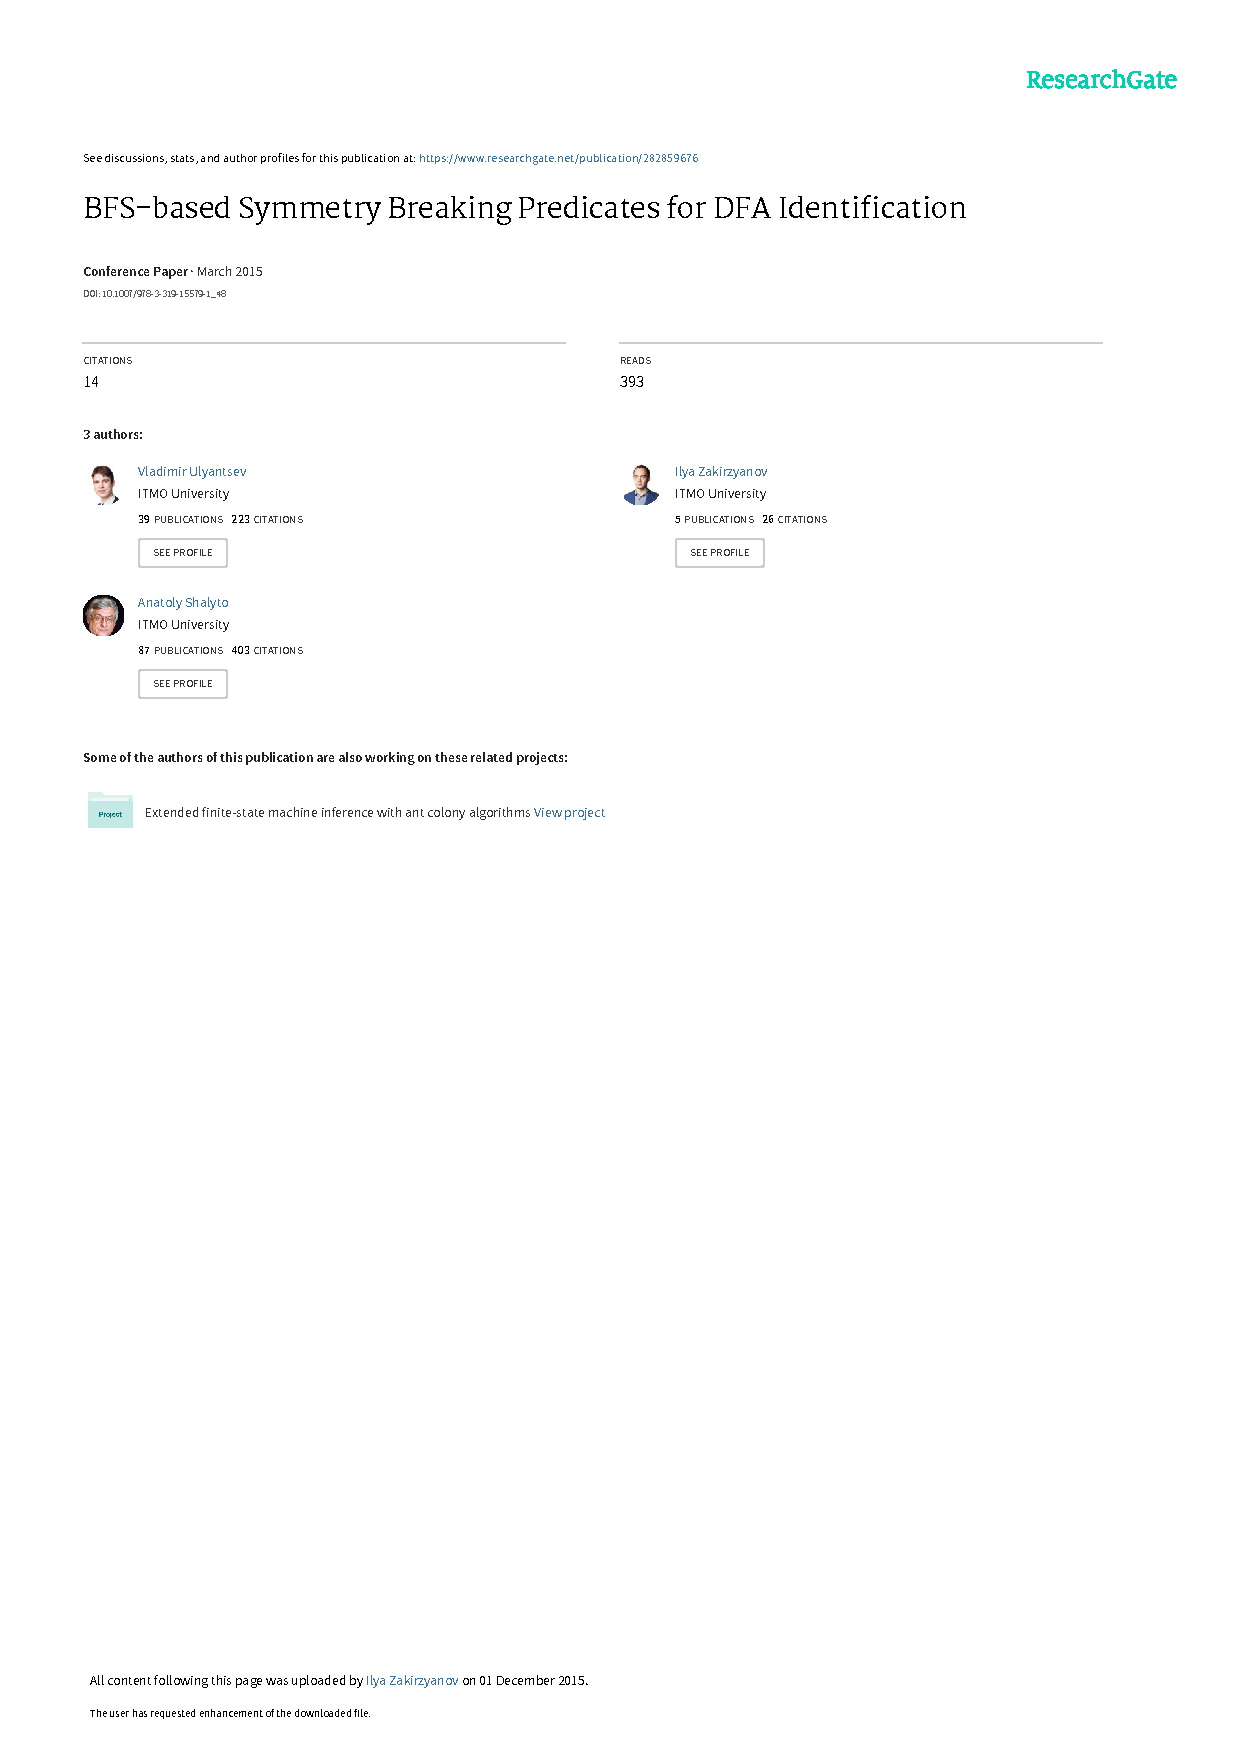
\includepdf[pages=-]{Papers/2015-LATA.pdf}
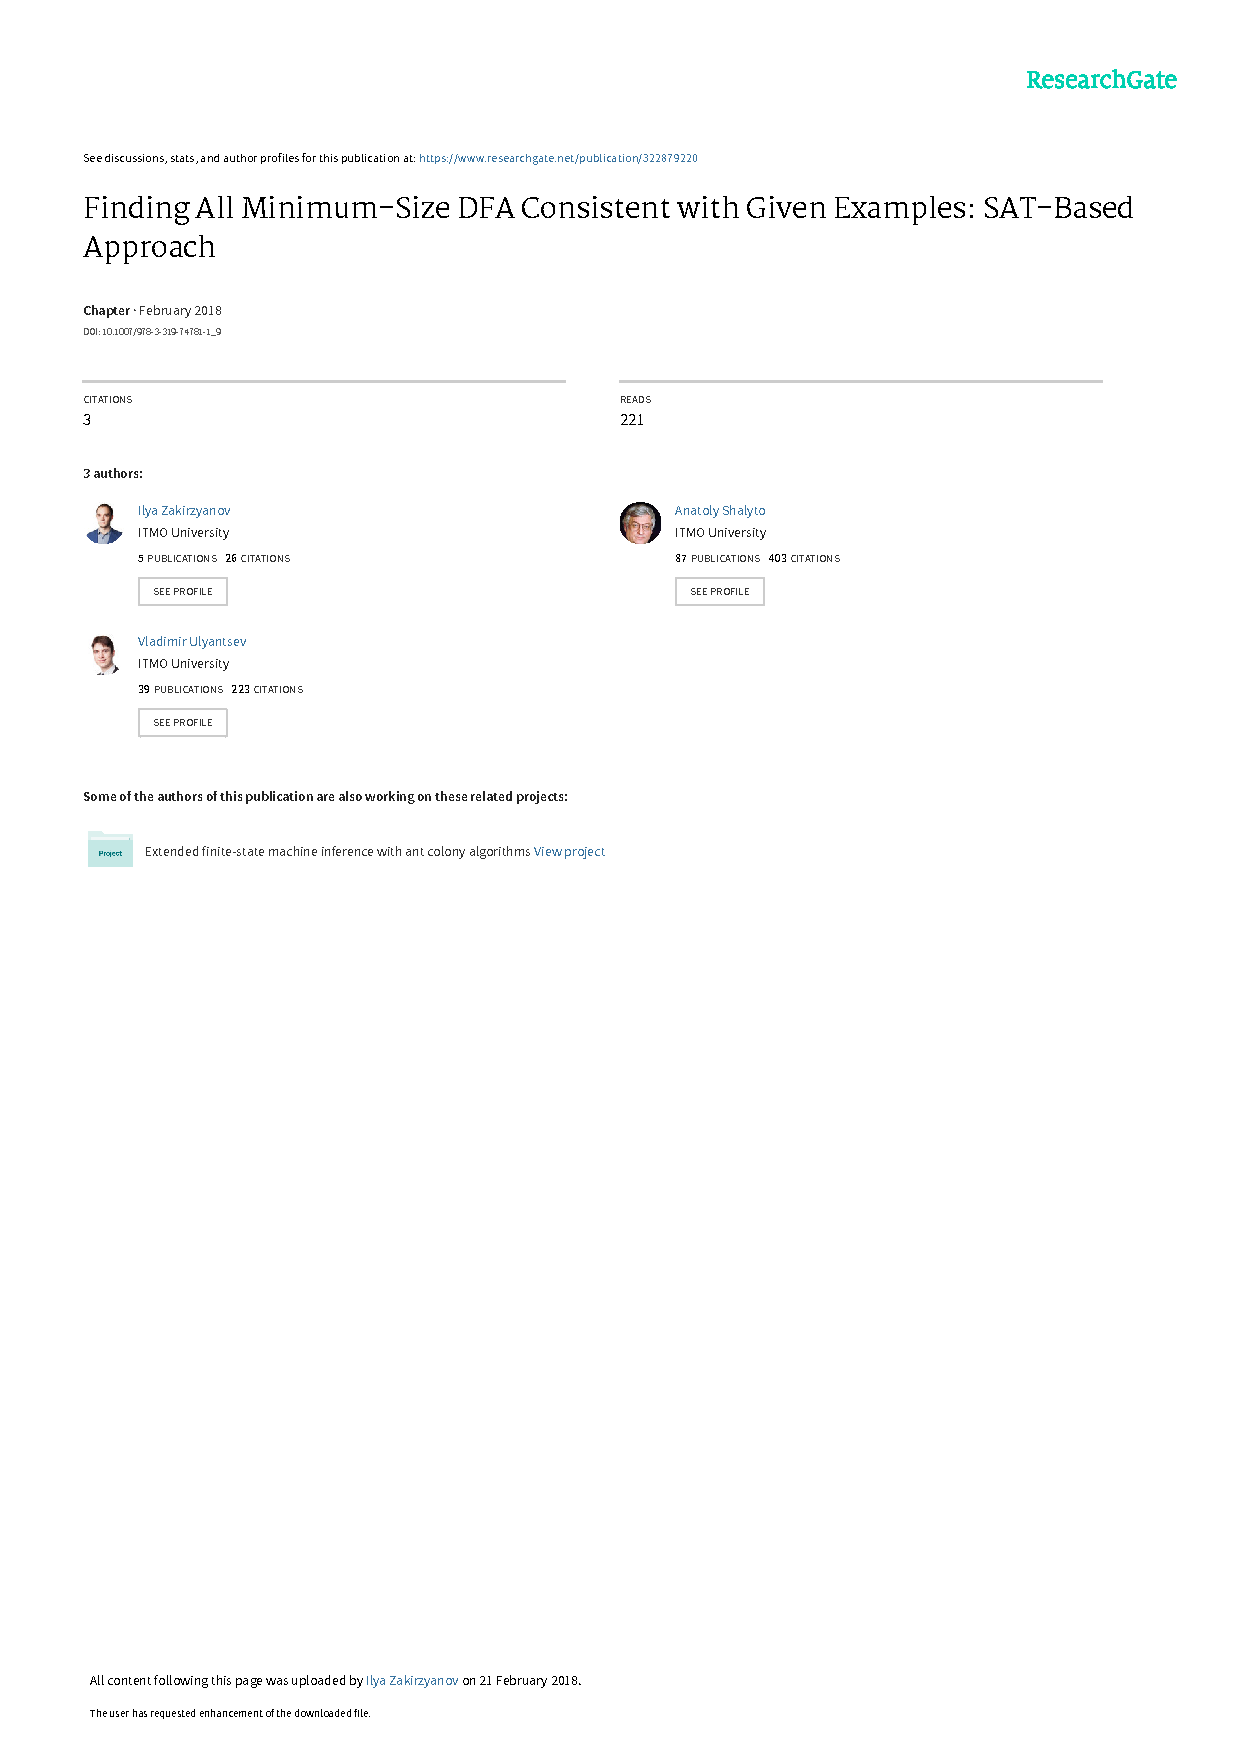
\includepdf[pages=-]{Papers/2017-DataMod.pdf}
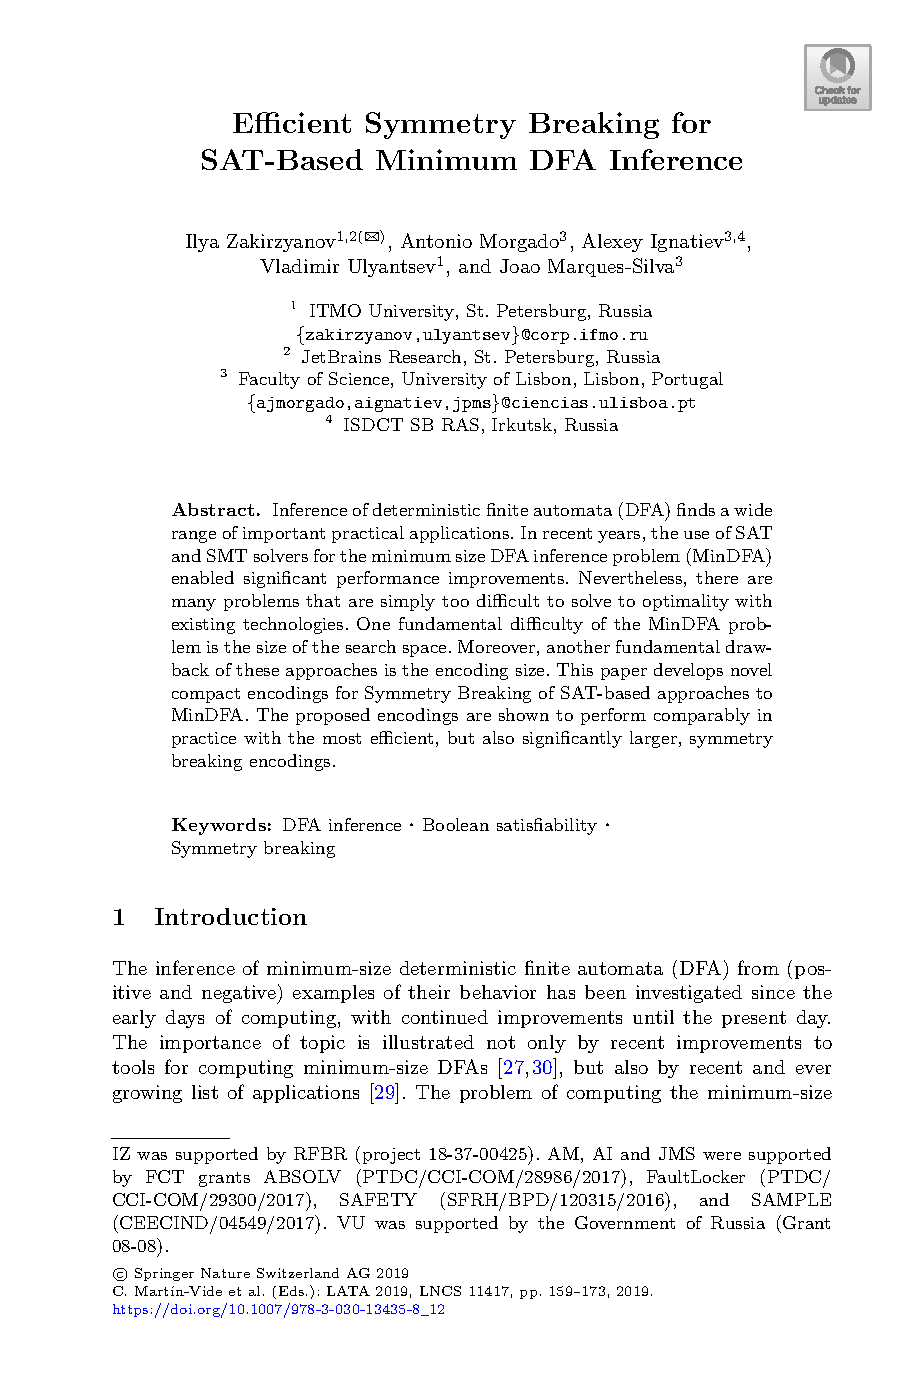
\includepdf[pages=-]{Papers/2019-LATA.pdf}
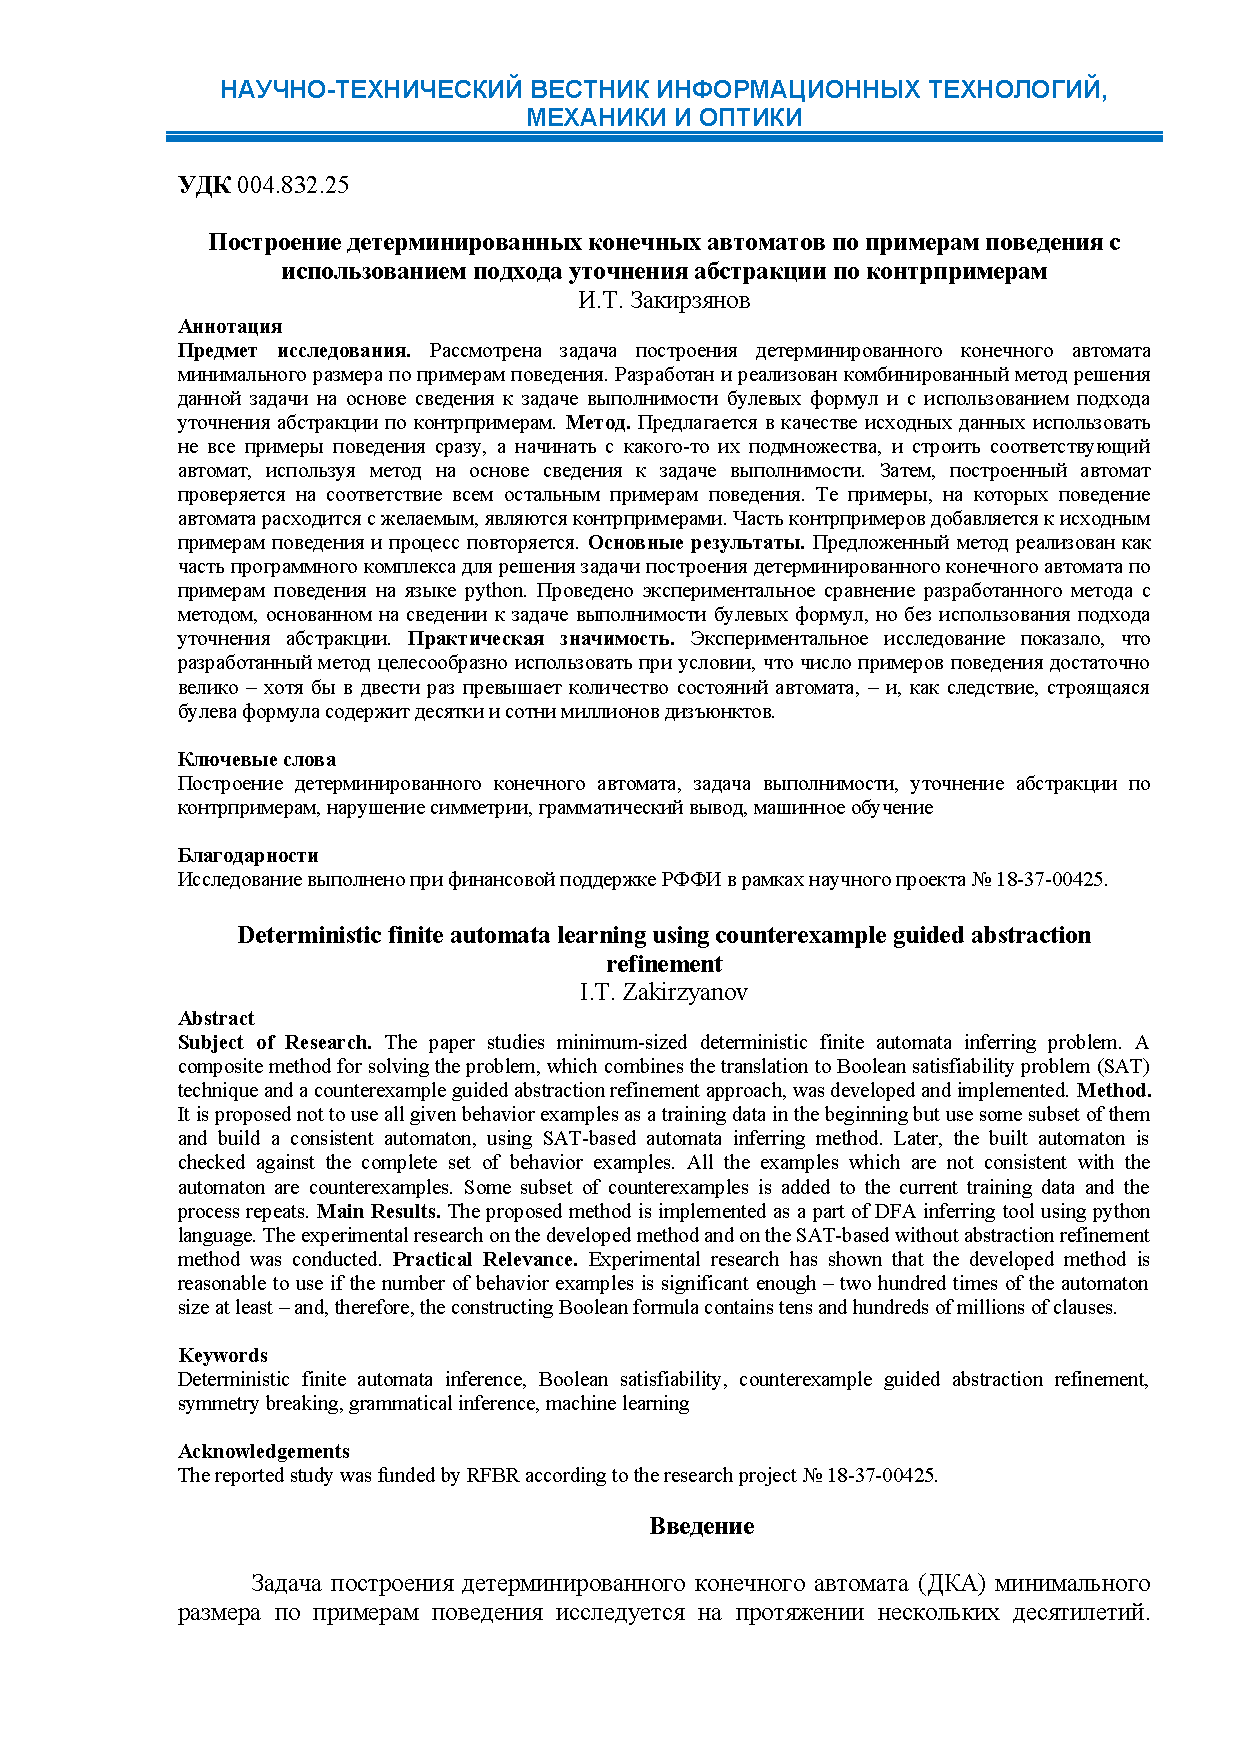
\includepdf[pages=-]{Papers/2020-Vestnik.pdf}

\end{document}
